\documentclass[12pt]{article}
\usepackage{amsmath, amssymb, amsfonts, bm, graphicx, geometry, tabularx, booktabs, float, enumitem}
\geometry{margin=1in}

\title{}
\date{}
\author{}

% Uppercase Volume - Wrapped in \mathord to prevent shifting
\newcommand{\vol}{\mathord{\text{\ooalign{\hidewidth $V$\hidewidth\cr\kern-1.0pt--}}}}

% Lowercase Volume - Adjusted for math mode stability
\newcommand{\svol}{\mathord{\text{\ooalign{\hidewidth $v$\hidewidth\cr\kern-0.2pt\raisebox{-0.1ex}{--}}}}}
\begin{document}

\section*{2-17}
\vspace{-1em}
\begin{minipage}[t]{0.6\textwidth} \vspace{0pt}
\centering
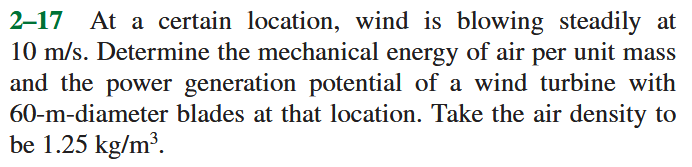
\includegraphics[width=\textwidth]{2-17.png}
\end{minipage}
\hfill
\begin{minipage}[t]{0.4\textwidth} \vspace{0pt}
Given:
\begin{itemize}
    \item Wind speed: $v=10$ m/s
    \item Turbine blade diameter: $d=60$ m
    \item Air density: $\rho=1.25$ kg/m$^3$
\end{itemize}
Find: 
\begin{itemize}
    \item Mechanical energy of air per unit mass
    \item Power generation potential of the wind turbine
\end{itemize}
\end{minipage}\\\\
\textbf{Power generation potential} refers to the \textit{maximum} amount of power that can be generated by the wind turbine. This occurs if all the kinetic energy of the wind is converted into rotational energy of the turbine blades. Thus, the mechanical energy of the air per unit mass is:
\[E_{\text{mech}} = \frac{1}{2}mv^2 \implies e_{\text{mech}} = \frac{1}{2}v^2\]
\[e_{\text{mech}} = \frac{1}{2} \left[10\,\frac{m}{s}\right]^2 = \left[50\,\frac{m^2}{s^2}\right] \left[\frac{J}{N\cdot m}\right]\left[\frac{N}{kg\cdot m/s^2}\right] = \boxed{50\,\frac{J}{kg}}\]
Power is the \textit{rate} of energy transfer or $\dot{W}$. Thus, multiplying the mechanical energy per unit mass by the mass flow rate $\dot{m}$ gives us energy per unit time, or power:
\[\boxed{\dot{W} = \dot{m} e_{\text{mech}},\quad \dot{m}= \rho v A}\]
\[\dot{W} = \rho v A \cdot \frac{1}{2}v^2 = \frac{1}{2} \rho A v^3 = \frac{1}{2} \left[1.25\,\frac{kg}{m^3}\right] \left[\frac{\pi}{4}(60\,m)^2\right] \left[10\,\frac{m}{s}\right]^3\]
\[\dot{W}= \left[1767145.86\,\frac{kg\cdot m^3}{s^3}\right] \left[\frac{J}{\frac{kg\cdot m^2}{s^2}}\right] = \boxed{1767 \times 10^3\, \frac{J}{s}}\]
We can also find $\dot{W}$ by applying the first law of thermodynamics to the control volume (open system) around the turbine blades:
\[\boxed{\frac{dE}{dt} = \dot{Q}-\dot{W}+\sum \dot{m_i}\left[h_i+\frac{1}{2}v_i^2+g z_i\right]-\sum \dot{m_e}\left[h_e+\frac{1}{2}v_e^2+g z_e\right]}\]
Where:
\begin{itemize}
\item $dE/dt$ is the rate of change of the total energy of the system over time
\item $\dot{Q}$ is the rate of heat transfer into the system from the surroundings
\item $\dot{W}$ is the rate of work done by the system on its surroundings (power output)
\item The summations represent the total energy entering and leaving the system due to mass flow, where $h$ is the specific enthalpy, $v/2$ is the specific kinetic energy, and $gz$ is the specific potential energy at the inlet ($i$) and outlet ($e$) of the control volume.
\end{itemize}
Assuming steady state $dE/dt = 0$, no heat transfer $\dot{Q}=0$ (adiabatic process, thus $h_i = h_e$), negligible change in potential energy ($z_i \approx z_e$), and that air stops completely at the turbine blades ($v_e = 0$), we can simplify the equation to:
\[\dot{W} = \sum \dot{m_i}\left[h_i+\frac{1}{2}v_i^2\right]-\sum \dot{m_e}\left[h_e\right] = \dot{m} \cdot \frac{1}{2}v^2\]
The same result as before.

\section*{2-30E}
\vspace{-1em}
\begin{minipage}[t]{0.6\textwidth} \vspace{0pt}
\centering
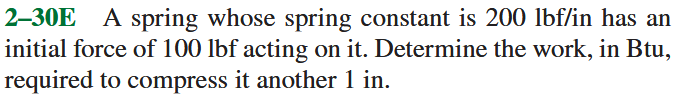
\includegraphics[width=\textwidth]{2-30E.png}
\end{minipage}
\hfill
\begin{minipage}[t]{0.4\textwidth} \vspace{0pt}
Given:
\begin{itemize}
    \item $k=200 lbf/in$
    \item $F_0 = 100 lbf$
\end{itemize}
Find: 
\begin{itemize}
    \item Work in Btw to compress the spring 1 more inch
\end{itemize}
\end{minipage}\\\\
\[F=kx_0 \implies x_0 = \frac{F_0}{k} = \frac{100\,lbf}{200\,\frac{lbf}{in}} = 0.5\,in\]
\[\Delta U_s = \frac{1}{2} k x_f^2 - \frac{1}{2} k x_0^2 = \frac{1}{2}\left[200\,\frac{lbf}{in}\right] \left[1.5\,in\right]^2 - \frac{1}{2}\left[200\,\frac{lbf}{in}\right] \left[0.5\,in\right]^2 = 200\,lbf \cdot in\]
\[[200\,lbf \cdot in]\left[\frac{ft}{12 in}\right]\left[\frac{Btu}{778.17\,ft \cdot lbf}\right] = \boxed{0.0214\, Btu}\]
\underline{Note:} $1\,Btu$ = $778.17\,ft \cdot lbf$ = $1055.06\,J$

\section*{2-45E}
\vspace{-1em}
\begin{minipage}[t]{0.6\textwidth} \vspace{0pt}
\centering
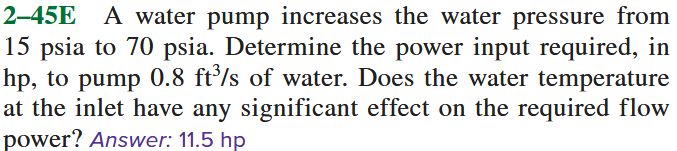
\includegraphics[width=\textwidth]{2-45E.png}
\end{minipage}
\hfill
\begin{minipage}[t]{0.4\textwidth} \vspace{0pt}
Given:
\begin{itemize}
    \item Input pressure: $P_i = 15$ psia
    \item Output pressure: $P_e = 70$ psia
    \item Volume flow rate $\dot{\vol} = 0.8 ft^3/s$
\end{itemize}
Find: 
\begin{itemize}
    \item Input power required in Hp
    \item Is the water temp at the inlet negligable?
\end{itemize}
\end{minipage}\\\\
\underline{Note:} Psia means pounds per square inch absolute, which is the pressure relative to a perfect vacuum. \\\\
Using flow power formula
\[\boxed{\dot{W} = \dot{\vol} (P_e - P_i)}\]
\[ \dot{W}= \left[0.8\frac{ft^3}{s}\right]\left[70-15\,\frac{lbf}{in^2}\right]\left[\frac{(12\,in)^2}{ft^2}\right] = 6336\,\frac{lbf\cdot ft}{s}\]
\[\left[6336\,\frac{lbf\cdot ft}{s}\right]\left[\frac{hp}{550\,\frac{lbf\cdot ft}{s}}\right] = \boxed{11.52\,hp}\]
\underline{Note:} $1\,hp$ = $550\,\frac{lbf\cdot ft}{s}$ = $745.7\,W$

\section*{2-92}
\vspace{-1em}
\begin{minipage}[t]{0.6\textwidth} \vspace{0pt}
\centering
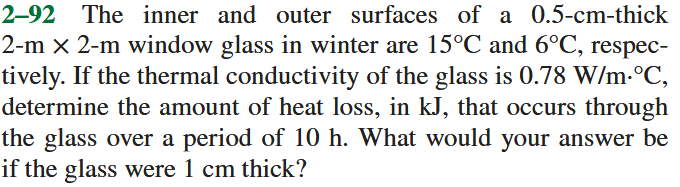
\includegraphics[width=\textwidth]{2-92.png}
\end{minipage}
\hfill
\begin{minipage}[t]{0.4\textwidth} \vspace{0pt}
Given:
\begin{itemize}
    \item Thickness of window $\Delta x=0.5$ cm
    \item Area of window 2 m $\times$ 2 m
    \item Temp inside $T_i = 15^\circ C$
    \item Temp outside $T_e = 6^\circ C$
    \item Thermal conductivity of glass $k=0.78$ W/m$\cdot ^\circ C$
\end{itemize}
Find: 
\begin{itemize}
    \item Find heat loss in kJ over 10 hrs
    \item Find heat loss is thickness is 1 cm
\end{itemize}
\end{minipage}\\\\
Heat conduction formula
\[\boxed{\dot{Q}_{\text{cond}} = kA\frac{\Delta T}{\Delta x}}\]
Where: $\Delta T = T_i - T_e$, $A$ is the area of the window, $k$ is the thermal conductivity of the material, and $\Delta x$ is the thickness of the window.
\[\dot{Q} = \left[0.78\,\frac{W}{m\cdot ^\circ C}\right]\left[4\,m^2\right]\frac{[15-6\, ^\circ C]}{[0.005\,m]} = 5616\,W\]
\[\implies Q = \dot{Q}\Delta t = [5616\,W] [10\,hrs]\left[\frac{3600\,s}{1\,hr}\right] = \boxed{2.02 \times 10^8\,J}\]
Doubling the thickness $\Delta x$ to 1 cm halves the heat loss, so $Q = 1.01 \times 10^8\,J$

\section*{2-119}
\vspace{-1em}
\begin{minipage}[t]{0.6\textwidth} \vspace{0pt}
\centering
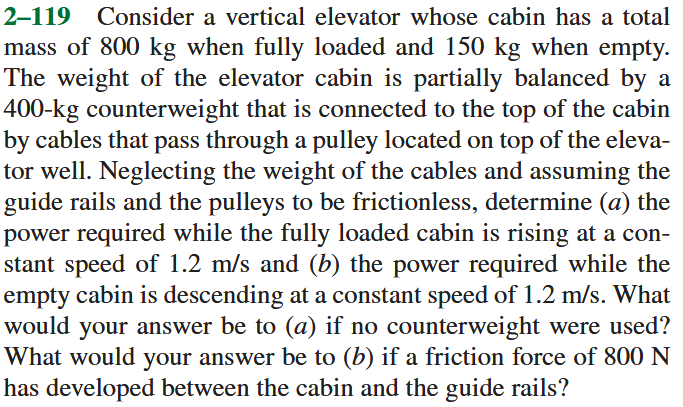
\includegraphics[width=\textwidth]{2-119.png}
\end{minipage}
\hfill
\begin{minipage}[t]{0.4\textwidth} \vspace{0pt}
Given:
\begin{itemize}
    \item $m_{\text{full}} = 800$ kg
    \item $m_{\text{empty}} = 150$ kg
    \item $m_{\text{counterweight}} = 400$ kg
\end{itemize}
Find: 
\begin{itemize}
    \item a) Power required to lift the full elevator up at 1.2 m/s
    \item b) Power required to lower the empty elevator down at 1.2 m/s
    \item What if no counterweight for a)
    \item What if there was friction of 800N for b)
\end{itemize}
\end{minipage}\\\\
\textbf{(a)}
\begin{center}
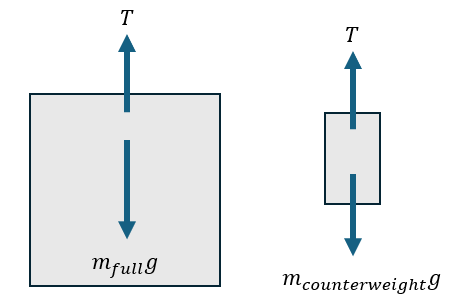
\includegraphics[width=0.5\textwidth]{2-119-1.png}
\end{center}
\[\implies T = m_{\text{counterweight}} g\]
\[\sum F_y = m_{\text{full}} g- m_{\text{counterweight}} g= [800\,kg]\left[9.81\,\frac{m}{s^2}\right] - [400\,kg]\left[9.81\,\frac{m}{s^2}\right] = 3924\,N\]
\[\dot{W} = F \cdot v = [3924\,N][1.2\,\frac{m}{s}] = \boxed{4708.8\,W}\]
\textbf{(b)}
\[\sum F_y = m_{\text{empty}} g - m_{\text{counterweight}} g= [150\,kg]\left[9.81\,\frac{m}{s^2}\right] - [400\,kg]\left[9.81\,\frac{m}{s^2}\right] = -2452.5\,N\]
\[\dot{W} = F \cdot v = [-2452.5\,N][1.2\,\frac{m}{s}] = \boxed{-2943\,W}\]
\textbf{No counterweight for a)}
\[\implies F = 7848\,N\]
\[\dot{W} = F \cdot v = [7848\,N][1.2\,\frac{m}{s}] = \boxed{9417.6\,W}\]
\textbf{Friction of 800N for b)}
\[\sum F_y = m_{\text{empty}} g - m_{\text{counterweight}} g - F_f = [150\,kg]\left[9.81\,\frac{m}{s^2}\right] - [400\,kg]\left[9.81\,\frac{m}{s^2}\right] - [800\,N] = -3252.5\,N\]
\[\dot{W} = F \cdot v = [-3252.5\,N][1.2\,\frac{m}{s}] = \boxed{-3903\,W}\]

\section*{2-129}
\vspace{-1em}
\begin{minipage}[t]{0.6\textwidth} \vspace{0pt}
\centering
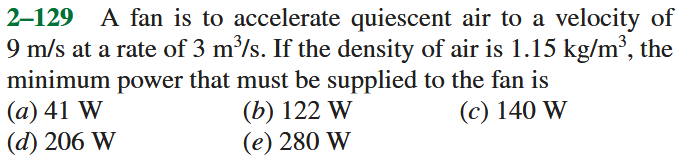
\includegraphics[width=\textwidth]{2-129.png}
\end{minipage}
\hfill
\begin{minipage}[t]{0.4\textwidth} \vspace{0pt}
Given:
\begin{itemize}
    \item $v = 9$ m/s
    \item Volume flow rate $\dot{\vol} = 3$ m$^3$/s
    \item Density $\rho = 1.15$ kg/m$^3$
\end{itemize}
Find: 
\begin{itemize}
    \item Min power supplied to the fan
\end{itemize}
\end{minipage}\\\\
Like problem 2-17,
\[\dot{W} = \dot{m}e_{\text{mech}} = \frac{1}{2}\rho \dot{V} v^2\]
\[\dot{W} = \frac{1}{2} [1.15\,\frac{kg}{m^3}] [3\,m^3/s] [9\,m/s]^2 = \boxed{139.7\,W}\]

\end{document}